
%% bare_conf.tex
%% V1.3
%% 2007/01/11
%% by Michael Shell
%% See:
%% http://www.michaelshell.org/
%% for current contact information.
%%
%% This is a skeleton file demonstrating the use of IEEEtran.cls
%% (requires IEEEtran.cls version 1.7 or later) with an IEEE conference paper.
%%
%% Support sites:
%% http://www.michaelshell.org/tex/ieeetran/
%% http://www.ctan.org/tex-archive/macros/latex/contrib/IEEEtran/
%% and
%% http://www.ieee.org/

%%*************************************************************************
%% Legal Notice:
%% This code is offered as-is without any warranty either expressed or
%% implied; without even the implied warranty of MERCHANTABILITY or
%% FITNESS FOR A PARTICULAR PURPOSE! 
%% User assumes all risk.
%% In no event shall IEEE or any contributor to this code be liable for
%% any damages or losses, including, but not limited to, incidental,
%% consequential, or any other damages, resulting from the use or misuse
%% of any information contained here.
%%
%% All comments are the opinions of their respective authors and are not
%% necessarily endorsed by the IEEE.
%%
%% This work is distributed under the LaTeX Project Public License (LPPL)
%% ( http://www.latex-project.org/ ) version 1.3, and may be freely used,
%% distributed and modified. A copy of the LPPL, version 1.3, is included
%% in the base LaTeX documentation of all distributions of LaTeX released
%% 2003/12/01 or later.
%% Retain all contribution notices and credits.
%% ** Modified files should be clearly indicated as such, including  **
%% ** renaming them and changing author support contact information. **
%%
%% File list of work: IEEEtran.cls, IEEEtran_HOWTO.pdf, bare_adv.tex,
%%                    bare_conf.tex, bare_jrnl.tex, bare_jrnl_compsoc.tex
%%*************************************************************************

% *** Authors should verify (and, if needed, correct) their LaTeX system  ***
% *** with the testflow diagnostic prior to trusting their LaTeX platform ***
% *** with production work. IEEE's font choices can trigger bugs that do  ***
% *** not appear when using other class files.                            ***
% The testflow support page is at:
% http://www.michaelshell.org/tex/testflow/



% Note that the a4paper option is mainly intended so that authors in
% countries using A4 can easily print to A4 and see how their papers will
% look in print - the typesetting of the document will not typically be
% affected with changes in paper size (but the bottom and side margins will).
% Use the testflow package mentioned above to verify correct handling of
% both paper sizes by the user's LaTeX system.
%
% Also note that the "draftcls" or "draftclsnofoot", not "draft", option
% should be used if it is desired that the figures are to be displayed in
% draft mode.
%
%\documentclass[conference]{IEEEtran}
\documentclass[conference,a4paper]{IEEEtran}
% Add the compsoc option for Computer Society conferences.
%
% If IEEEtran.cls has not been installed into the LaTeX system files,
% manually specify the path to it like:
% \documentclass[conference]{../sty/IEEEtran}





% Some very useful LaTeX packages include:
% (uncomment the ones you want to load)


% *** MISC UTILITY PACKAGES ***
%
%\usepackage{ifpdf}
% Heiko Oberdiek's ifpdf.sty is very useful if you need conditional
% compilation based on whether the output is pdf or dvi.
% usage:
% \ifpdf
%   % pdf code
% \else
%   % dvi code
% \fi
% The latest version of ifpdf.sty can be obtained from:
% http://www.ctan.org/tex-archive/macros/latex/contrib/oberdiek/
% Also, note that IEEEtran.cls V1.7 and later provides a builtin
% \ifCLASSINFOpdf conditional that works the same way.
% When switching from latex to pdflatex and vice-versa, the compiler may
% have to be run twice to clear warning/error messages.






% *** CITATION PACKAGES ***
%
%\usepackage{cite}
% cite.sty was written by Donald Arseneau
% V1.6 and later of IEEEtran pre-defines the format of the cite.sty package
% \cite{} output to follow that of IEEE. Loading the cite package will
% result in citation numbers being automatically sorted and properly
% "compressed/ranged". e.g., [1], [9], [2], [7], [5], [6] without using
% cite.sty will become [1], [2], [5]--[7], [9] using cite.sty. cite.sty's
% \cite will automatically add leading space, if needed. Use cite.sty's
% noadjust option (cite.sty V3.8 and later) if you want to turn this off.
% cite.sty is already installed on most LaTeX systems. Be sure and use
% version 4.0 (2003-05-27) and later if using hyperref.sty. cite.sty does
% not currently provide for hyperlinked citations.
% The latest version can be obtained at:
% http://www.ctan.org/tex-archive/macros/latex/contrib/cite/
% The documentation is contained in the cite.sty file itself.






% *** GRAPHICS RELATED PACKAGES ***
%
\ifCLASSINFOpdf
  \usepackage[pdftex]{graphicx}
  % declare the path(s) where your graphic files are
  % \graphicspath{{../pdf/}{../jpeg/}}
  % and their extensions so you won't have to specify these with
  % every instance of \includegraphics
  % \DeclareGraphicsExtensions{.pdf,.jpeg,.png}
\else
  % or other class option (dvipsone, dvipdf, if not using dvips). graphicx
  % will default to the driver specified in the system graphics.cfg if no
  % driver is specified.
  % \usepackage[dvips]{graphicx}
  % declare the path(s) where your graphic files are
  % \graphicspath{{../eps/}}
  % and their extensions so you won't have to specify these with
  % every instance of \includegraphics
  % \DeclareGraphicsExtensions{.eps}
\fi
% graphicx was written by David Carlisle and Sebastian Rahtz. It is
% required if you want graphics, photos, etc. graphicx.sty is already
% installed on most LaTeX systems. The latest version and documentation can
% be obtained at: 
% http://www.ctan.org/tex-archive/macros/latex/required/graphics/
% Another good source of documentation is "Using Imported Graphics in
% LaTeX2e" by Keith Reckdahl which can be found as epslatex.ps or
% epslatex.pdf at: http://www.ctan.org/tex-archive/info/
%
% latex, and pdflatex in dvi mode, support graphics in encapsulated
% postscript (.eps) format. pdflatex in pdf mode supports graphics
% in .pdf, .jpeg, .png and .mps (metapost) formats. Users should ensure
% that all non-photo figures use a vector format (.eps, .pdf, .mps) and
% not a bitmapped formats (.jpeg, .png). IEEE frowns on bitmapped formats
% which can result in "jaggedy"/blurry rendering of lines and letters as
% well as large increases in file sizes.
%
% You can find documentation about the pdfTeX application at:
% http://www.tug.org/applications/pdftex





% *** MATH PACKAGES ***
%
\usepackage[cmex10]{amsmath}
% A popular package from the American Mathematical Society that provides
% many useful and powerful commands for dealing with mathematics. If using
% it, be sure to load this package with the cmex10 option to ensure that
% only type 1 fonts will utilized at all point sizes. Without this option,
% it is possible that some math symbols, particularly those within
% footnotes, will be rendered in bitmap form which will result in a
% document that can not be IEEE Xplore compliant!
%
% Also, note that the amsmath package sets \interdisplaylinepenalty to 10000
% thus preventing page breaks from occurring within multiline equations. Use:
%\interdisplaylinepenalty=2500
% after loading amsmath to restore such page breaks as IEEEtran.cls normally
% does. amsmath.sty is already installed on most LaTeX systems. The latest
% version and documentation can be obtained at:
% http://www.ctan.org/tex-archive/macros/latex/required/amslatex/math/





% *** SPECIALIZED LIST PACKAGES ***
%
%\usepackage{algorithmic}
% algorithmic.sty was written by Peter Williams and Rogerio Brito.
% This package provides an algorithmic environment fo describing algorithms.
% You can use the algorithmic environment in-text or within a figure
% environment to provide for a floating algorithm. Do NOT use the algorithm
% floating environment provided by algorithm.sty (by the same authors) or
% algorithm2e.sty (by Christophe Fiorio) as IEEE does not use dedicated
% algorithm float types and packages that provide these will not provide
% correct IEEE style captions. The latest version and documentation of
% algorithmic.sty can be obtained at:
% http://www.ctan.org/tex-archive/macros/latex/contrib/algorithms/
% There is also a support site at:
% http://algorithms.berlios.de/index.html
% Also of interest may be the (relatively newer and more customizable)
% algorithmicx.sty package by Szasz Janos:
% http://www.ctan.org/tex-archive/macros/latex/contrib/algorithmicx/




% *** ALIGNMENT PACKAGES ***
%
%\usepackage{array}
% Frank Mittelbach's and David Carlisle's array.sty patches and improves
% the standard LaTeX2e array and tabular environments to provide better
% appearance and additional user controls. As the default LaTeX2e table
% generation code is lacking to the point of almost being broken with
% respect to the quality of the end results, all users are strongly
% advised to use an enhanced (at the very least that provided by array.sty)
% set of table tools. array.sty is already installed on most systems. The
% latest version and documentation can be obtained at:
% http://www.ctan.org/tex-archive/macros/latex/required/tools/


%\usepackage{mdwmath}
%\usepackage{mdwtab}
% Also highly recommended is Mark Wooding's extremely powerful MDW tools,
% especially mdwmath.sty and mdwtab.sty which are used to format equations
% and tables, respectively. The MDWtools set is already installed on most
% LaTeX systems. The lastest version and documentation is available at:
% http://www.ctan.org/tex-archive/macros/latex/contrib/mdwtools/


% IEEEtran contains the IEEEeqnarray family of commands that can be used to
% generate multiline equations as well as matrices, tables, etc., of high
% quality.


%\usepackage{eqparbox}
% Also of notable interest is Scott Pakin's eqparbox package for creating
% (automatically sized) equal width boxes - aka "natural width parboxes".
% Available at:
% http://www.ctan.org/tex-archive/macros/latex/contrib/eqparbox/





% *** SUBFIGURE PACKAGES ***
%\usepackage[tight,footnotesize]{subfigure}
% subfigure.sty was written by Steven Douglas Cochran. This package makes it
% easy to put subfigures in your figures. e.g., "Figure 1a and 1b". For IEEE
% work, it is a good idea to load it with the tight package option to reduce
% the amount of white space around the subfigures. subfigure.sty is already
% installed on most LaTeX systems. The latest version and documentation can
% be obtained at:
% http://www.ctan.org/tex-archive/obsolete/macros/latex/contrib/subfigure/
% subfigure.sty has been superceeded by subfig.sty.



%\usepackage[caption=false]{caption}
%\usepackage[font=footnotesize]{subfig}
% subfig.sty, also written by Steven Douglas Cochran, is the modern
% replacement for subfigure.sty. However, subfig.sty requires and
% automatically loads Axel Sommerfeldt's caption.sty which will override
% IEEEtran.cls handling of captions and this will result in nonIEEE style
% figure/table captions. To prevent this problem, be sure and preload
% caption.sty with its "caption=false" package option. This is will preserve
% IEEEtran.cls handing of captions. Version 1.3 (2005/06/28) and later 
% (recommended due to many improvements over 1.2) of subfig.sty supports
% the caption=false option directly:
%\usepackage[caption=false,font=footnotesize]{subfig}
%
% The latest version and documentation can be obtained at:
% http://www.ctan.org/tex-archive/macros/latex/contrib/subfig/
% The latest version and documentation of caption.sty can be obtained at:
% http://www.ctan.org/tex-archive/macros/latex/contrib/caption/




% *** FLOAT PACKAGES ***
%
%\usepackage{fixltx2e}
% fixltx2e, the successor to the earlier fix2col.sty, was written by
% Frank Mittelbach and David Carlisle. This package corrects a few problems
% in the LaTeX2e kernel, the most notable of which is that in current
% LaTeX2e releases, the ordering of single and double column floats is not
% guaranteed to be preserved. Thus, an unpatched LaTeX2e can allow a
% single column figure to be placed prior to an earlier double column
% figure. The latest version and documentation can be found at:
% http://www.ctan.org/tex-archive/macros/latex/base/



%\usepackage{stfloats}
% stfloats.sty was written by Sigitas Tolusis. This package gives LaTeX2e
% the ability to do double column floats at the bottom of the page as well
% as the top. (e.g., "\begin{figure*}[!b]" is not normally possible in
% LaTeX2e). It also provides a command:
%\fnbelowfloat
% to enable the placement of footnotes below bottom floats (the standard
% LaTeX2e kernel puts them above bottom floats). This is an invasive package
% which rewrites many portions of the LaTeX2e float routines. It may not work
% with other packages that modify the LaTeX2e float routines. The latest
% version and documentation can be obtained at:
% http://www.ctan.org/tex-archive/macros/latex/contrib/sttools/
% Documentation is contained in the stfloats.sty comments as well as in the
% presfull.pdf file. Do not use the stfloats baselinefloat ability as IEEE
% does not allow \baselineskip to stretch. Authors submitting work to the
% IEEE should note that IEEE rarely uses double column equations and
% that authors should try to avoid such use. Do not be tempted to use the
% cuted.sty or midfloat.sty packages (also by Sigitas Tolusis) as IEEE does
% not format its papers in such ways.





% *** PDF, URL AND HYPERLINK PACKAGES ***
%
%\usepackage{url}
% url.sty was written by Donald Arseneau. It provides better support for
% handling and breaking URLs. url.sty is already installed on most LaTeX
% systems. The latest version can be obtained at:
% http://www.ctan.org/tex-archive/macros/latex/contrib/misc/
% Read the url.sty source comments for usage information. Basically,
% \url{my_url_here}.





% *** Do not adjust lengths that control margins, column widths, etc. ***
% *** Do not use packages that alter fonts (such as pslatex).         ***
% There should be no need to do such things with IEEEtran.cls V1.6 and later.
% (Unless specifically asked to do so by the journal or conference you plan
% to submit to, of course. )


% correct bad hyphenation here
\hyphenation{op-tical net-works semi-conduc-tor}


\begin{document}
%
% paper title
% can use linebreaks \\ within to get better formatting as desired
\title{Can we date an artist's work from catalogue photographs?}


% author names and affiliations
% use a multiple column layout for up to three different
% affiliations
\author{\IEEEauthorblockN{Alexander David Brown}
\IEEEauthorblockA{Department of Computer Science,\\
Llandinam Building,\\
Aberystwyth University,\\
Aberystwyth,\\
Ceredigion,\\
SY23 3DB\\
Email: adb9@aber.ac.uk}
\and
\IEEEauthorblockN{Gareth Lloyd Roderick}
\IEEEauthorblockA{\\
Email: glr7@aber.ac.uk}
\and
\IEEEauthorblockN{Hannah M. Dee}
\IEEEauthorblockA{Department of Computer Science,\\
Llandinam Building,\\
Aberystwyth University,\\
Aberystwyth,\\
Ceredigion,\\
SY23 3DB\\
Email: hmd1@aber.ac.uk}
\and
\IEEEauthorblockN{Lorna M. Hughes}
\IEEEauthorblockA{\\
Email: lorna.hughes@llgc.org.uk}}

% conference papers do not typically use \thanks and this command
% is locked out in conference mode. If really needed, such as for
% the acknowledgment of grants, issue a \IEEEoverridecommandlockouts
% after \documentclass

% for over three affiliations, or if they all won't fit within the width
% of the page, use this alternative format:
% 
%\author{\IEEEauthorblockN{Michael Shell\IEEEauthorrefmark{1},
%Homer Simpson\IEEEauthorrefmark{2},
%James Kirk\IEEEauthorrefmark{3}, 
%Montgomery Scott\IEEEauthorrefmark{3} and
%Eldon Tyrell\IEEEauthorrefmark{4}}
%\IEEEauthorblockA{\IEEEauthorrefmark{1}School of Electrical and Computer Engineering\\
%Georgia Institute of Technology,
%Atlanta, Georgia 30332--0250\\ Email: see http://www.michaelshell.org/contact.html}
%\IEEEauthorblockA{\IEEEauthorrefmark{2}Twentieth Century Fox, Springfield, USA\\
%Email: homer@thesimpsons.com}
%\IEEEauthorblockA{\IEEEauthorrefmark{3}Starfleet Academy, San Francisco, California 96678-2391\\
%Telephone: (800) 555--1212, Fax: (888) 555--1212}
%\IEEEauthorblockA{\IEEEauthorrefmark{4}Tyrell Inc., 123 Replicant Street, Los Angeles, California 90210--4321}}




% use for special paper notices
%\IEEEspecialpapernotice{(Invited Paper)}




% make the title area
\maketitle


\begin{abstract}
%\boldmath
Kyffin Williams, art changes over time, blah blah blah. Features, colour, edges, histograms of oriented gradients; strong correlation using leave-one-out methodology.
Exemplars; artistic and statistic. 
\end{abstract}
% IEEEtran.cls defaults to using nonbold math in the Abstract.
% This preserves the distinction between vectors and scalars. However,
% if the conference you are submitting to favors bold math in the abstract,
% then you can use LaTeX's standard command \boldmath at the very start
% of the abstract to achieve this. Many IEEE journals/conferences frown on
% math in the abstract anyway.

% no keywords




% For peer review papers, you can put extra information on the cover
% page as needed:
% \ifCLASSOPTIONpeerreview
% \begin{center} \bfseries EDICS Category: 3-BBND \end{center}
% \fi
%
% For peerreview papers, this IEEEtran command inserts a page break and
% creates the second title. It will be ignored for other modes.
\IEEEpeerreviewmaketitle



\section{Introduction}
% no \IEEEPARstart
% You must have at least 2 lines in the paragraph with the drop letter
% (should never be an issue)

This paper presents a interdisciplinary computational study into the modelling
of artistic style, and how this style changes over time. The artist Sir John
(Kyffin) Williams painted from X to 2004, and produced a good many paintings
during this period -- he was a prolific painter. His style evolved from a very
figurative, representational style, to something more abstract: the computer
scientists on our team would say that the paintings became more \emph{blocky};
the art historians that \emph{XXXwhatever lorna and lloyd want to say}. Through
a collection of digital photographs of oil paintings, collected from museum
websites, catalogues and other sources, we first investigate whether it is
possible to date a painting from an unknown year based upon image features
alone.  

XXX mention key features of Kyffin's work, Patagonia, where he painted


\section{Background}
% 1 Page on Lloyd's work

\subsection{A digital humanities approach to art history}

\subsection{Computer vision and the analysis of paintings}

%Stroke analysis is one of the main goals for this project. It is quite apparent from looking at 
%Kyffin Williams' paintings that his brush-strokes change over time, his early work having lots of
%smaller strokes over the canvas to large bold strokes in his later work.

\cite{Berezhnoy2005Authentic} defines a method of analysing brush-strokes by moving a circular filter
across the whole painting to find the ridges of strokes, then filling any unbroken areas. They then
shrunk these areas to a single pixel line and fitted a $n^{\text{th}}$ order polynomial to this
line. This method seems fairly simplistic, but could be an interesting first step, but as it is 
more focused on authenticating paintings it may be of limited use.

Another method for stroke analysis has been published in the IEEE Transactions on Pattern Analysis
and Machine Learning journal. This method is far more complex, but is able to extract and label
individual brush-strokes. An interesting part of their findings was the ability to date some of Van
Gogh's paintings to a known period in his career\cite{Li2012Rhythmic}.

This method involves performing edge detection of the painting followed by an edge linking 
algorithm which aims to remove small, noisy edges and to trace every edge. With this they then
perform enclosing, as strokes may not be complete this stage also aims to fill in missing gaps of
strokes and to fill these in within a certain tolerance.

The algorithm then decides if a stroke really is a painted stroke, if the stroke is completely 
enclosed, isolated from other non-edge pixels and forms a connected component then it is likely 
that it is a proper brush-stroke and is extracted. The edge pixels are used as the background and
the non-edge pixels as the foreground, this is the process of labelling the brush-stroke.

For each of these labelled candidates, a heuristic function is used to threshold any brush-strokes 
that are either too long or too short, these strokes are discarded. These strokes are then
considered to be candidates if they are not significantly branched, the stroke is not too wide 
(this may change for Kyffin Williams as he used a pallet knife rather than a brush) and the 
brush-stroke is not too big or small.

Separately, the image is then segmented using $k$-means clustering by RGB values. This clustering 
algorithm is applied several times, lowering the tolerances for distance within a cluster. 
Connected components as a result of this clustering and have noise reduction performed upon them.
Finally, the two types of brush-strokes are combined.

This technique may need some changing to account for Kyffin Williams' use of a pallet knife, but
the overall principals of this technique should work with Kyffin's paintings.

%XXX in here we will need refs to that work on van gogh, to the guy who wrote
%the review paper, and to anything else on computer analysis of paintings that
%is relevant. What we're looking for are 5+ references, going from the general
%(massive review paper) to the specific (image processing to analyse artistic
%style). Bonus points for freshness - we don't really want to cite anything
%older than 10 years. Can you copy and paste some stuff from your MPR? Doesn't
%matter if it's too long I'll hack it back.

\section{The image dataset}

Our image dataset consists of 325 paintings, with associated metadata. Metadata
includes title, year or year ranges (for those works where year is unknown but
can be estimated by curators), genre, original painting size, painting
materials and image size.

These photographs of paintings are challenging in and of themselves: they are
not colour calibrated; some suffer from reflections (towards the end of his
life Kyffin painted using exceptionally thick and textural strokes, which gives
specularities on the catalogue images); they are at varying resolutions; and
come from a range of different cameras. Image size bears little relation to the
original painting size, and some images are even optimised for the web.
Table~\ref{summary_t} below summarises the dataset

\begin{table}[h]
\begin{tabular}{| l | c | c | p{3cm} |}
Type & Number & Number & Notes \\
  & & (Known date) &  \\
\hline
Landscapes  & 247 & 64 & \\
Portraits   &  52 & 35 & \\
Seascapes   &  11 &  2 & \\
Still lifes &   4 &  1 & \\
Other       &   8 &  0 & Genre unknown or studies \\
\end{tabular}
\caption{A summary of the Kyffin Williams painting dataset used}
\label{summary_t}
\end{table}

XXXIt may be worth putting in something here about image size vs painting size?


\section{Methodology}
% 0.5 Page on the validation - LOOCV

Within our database of 325 paintings, we know the actual year of painting for
102 artworks. In order to determine the accuracy of our results, rather than
work with the full dataset (and work with images with uncertain metadata in the
form of date ranges), we have used a leave-one-out cross validation
methodology. This involves us taking a painting for which we know the year, and
then using our classifier to guess that year; thus we are able to tell whether
we are right. We are also able, if we are wrong, to determine exactly how wrong
we are.  

To simplify the classification stage we use a K-Nearest Neighbour (KNN)
classifier with the other 101 paintings for which we know the date. KNN is a
fast, non-parametric classifier which makes no assumptions about the underlying
patterns in the data, merely that paintings from around the same time will be
similarly located in our feature space(s). Whilst we suspect that there may be
some broader underlying trend in the change of style, for this work have
concentrated on features for classification rather than the question of
classification or regression itself. 
 
\begin{figure}
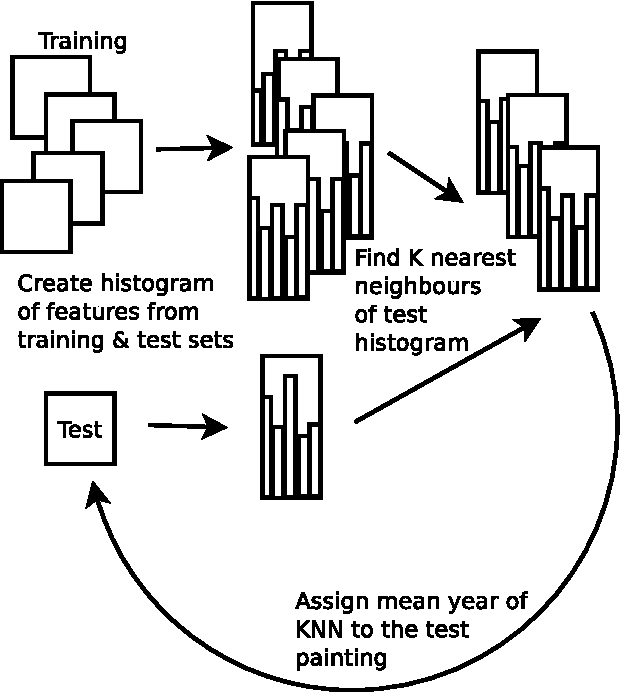
\includegraphics[width=8cm]{kyffin_overview.pdf}
\caption{Overview of the classification methodology}
\label{LOOCV}
\end{figure}
% yes diagram looks proper fuzzy but if we can work out export to pdf
% instead of png then it'll look ok. you should have the dia file as 
% well as the png

Thus for each feature set, we take all paintings for which we know the year of
creation; select one painting, and find its nearest neighbours within that
feature space. The year assigned by our classifier to that painting is the 
mean of the K neighbours.
Figure~\ref{LOOCV} provides an overview of this classification methodology.


We also know that painting's actual year, and we can plot actual against
predicted year for all known-year paintings.  To measure goodness of fit, the
Pearson's product-moment correlation coefficient was calculated on these
orderings; this provides us with a performance measure of each classifier.  It
is also possible to test Pearson's R for statistical significance; thus
significance levels are reported alongside R in this paper.

% XXX Thought: You can test Pearson's for statistical significance - can we try this?
% http://www.vassarstats.net/textbook/ch4apx.html 
% Should not require much change to your code.


\section{An exploration of colour and texture features}

% 0.5 page on references
% 4 pages on the rest

The digital analysis of paintings is a broad reseach area. Within the
methodology we have selected, there are many feature spaces which could be
useful: from simple analysis of the way in which colour changes over time,
through edge detection, to texture analysis and maybe even brush-stroke
recognition. Within this work we have concentrated on lower level image
features -- colours, textures, and edges -- rather than attempt to extract
brush strokes. Kyffin Williams painted with a pallette knife rather than a
brush, and his work is characterised by angularity rather than identifiable
``strokes''.

As there is a clear (to the eye) trend in colour usage, as the paintings get
``gloomier'' over time, we started with simple colour-space analysis: taking
the mean RGB for each painting and using this with our KNN classfier; we also
tested other colour spaces, such as HSV. Promisingly this provided us with a
positive correlation.  With all of these analysis techniques we treat the
results as histograms, this allows us to use a single distance measure, namely
chi-squared, for k-nearest neighbour.

Staying with the colour variation theme, we then used colour histograms, which
provide a more precise representation of the way Kyffin Williams used colour.
These histograms were developed by counting the number of pixels within a
particular colour range for each painting, and then building a normalised
histogram representing the colour usage.
 
As a lot of Kyffin Williams' paintings are highly textural, edge detection and
texture analysis were thought to be good techniques to explore.

Edge detection involved applying one of the various edge detection algorithms
available, applying it to each painting. The distance measure is base on the
number and strength of edges in the painting. Canny\cite{Canny1986Computational} 
edge detection is a reasonable algorithm for this. %TODO Why?

Texture analysis is a continuation of edge detection. Instead of just taking
the strength and number of edges, we create a histogram of orientated gradients
as in \cite{Dalal2005Histograms}. In this way we begin to build up a richer
representation of the texture of a painting. Given the change in style of
Kyffin Williams' work, moving away from figurative representations with curved
lines towards more blocky rectilinear brush strokes, we expect these edge
orientation frequencies to change over time. To this end we used simple
steerable filters $S$, applied to the image at $0$, $\frac{\pi}{4}$,
$\frac{\pi}{2}$ and $\frac{3\pi}{4}$. 
\begin{equation}
S\left(\frac{\pi}{2}\right) = \left( \begin{array}{ccc}
0 & 0 & 0 \\
1 & 1 & 1 \\
0 & 0 & 0 \end{array} \right)
\label{filter_ex}
\end{equation}

Equation~\ref{filter_ex} shows a sample steerable filter, in this case
$S(\frac{\pi}{2})$, the filter which gives the highest response when presented
with horizontal lines. By convolving each image with filters tuned to different
orientations, we can build a histogram recording the frequency of lines at each
orientation.

 XXX Can we have a visualisation of this? perhaps a picture with its associated
histogram? maybe a crop from this blog http://users.aber.ac.uk/adb9/?e=27 but
maybe we want to make the visualisation a bit more stand out...

Gabor filters were also used with a greater range of angles to produce a more
accurate representation of the texture of the painting.

\begin{equation}
g_e(x) = \frac{1}{2\pi\sigma_x \sigma_y}e^{-\frac{1}{2}\left(\frac{x^2}{\sigma_x}+\frac{y^2}{\sigma_y}\right)}\cos(2\pi\omega_{x_0}x + 2\pi\omega_{y_0}y)
\label{gabor_eq}
\end{equation}

Where $(\omega_{x_0},\omega_{y_0})$\ defines the centre frequency, and
$(\sigma_x,\sigma_y)$ the spread of the Gaussian window.


 XXX Again, can we get a visualisation? What does Gabor give us that steerable 
filters don't (apart from scary mathematics?)

Another method for producing histograms of orientated gradients is to apply two
discrete derivative masks to the image to get the gradient of $x$ and $y$ and
then to work out the gradient direction at each point. This can then have a
histogram created from it to provide a different representation of the texture
of the image.

% XXX Right oh now what we need is some graphs
% I suggest for now doing results in-line, or have a table here showing 
% correlation coefficients 

\begin{figure}[h]
\centering
% GNUPLOT: LaTeX picture
\setlength{\unitlength}{0.240900pt}
\ifx\plotpoint\undefined\newsavebox{\plotpoint}\fi
\sbox{\plotpoint}{\rule[-0.200pt]{0.400pt}{0.400pt}}%
\begin{picture}(900,540)(0,0)
\sbox{\plotpoint}{\rule[-0.200pt]{0.400pt}{0.400pt}}%
\put(171.0,131.0){\rule[-0.200pt]{4.818pt}{0.400pt}}
\put(151,131){\makebox(0,0)[r]{ 0}}
\put(819.0,131.0){\rule[-0.200pt]{4.818pt}{0.400pt}}
\put(171.0,315.0){\rule[-0.200pt]{4.818pt}{0.400pt}}
\put(151,315){\makebox(0,0)[r]{ 0.1}}
\put(819.0,315.0){\rule[-0.200pt]{4.818pt}{0.400pt}}
\put(171.0,499.0){\rule[-0.200pt]{4.818pt}{0.400pt}}
\put(151,499){\makebox(0,0)[r]{ 0.2}}
\put(819.0,499.0){\rule[-0.200pt]{4.818pt}{0.400pt}}
\put(171.0,131.0){\rule[-0.200pt]{0.400pt}{4.818pt}}
\put(171,90){\makebox(0,0){ 0}}
\put(171.0,479.0){\rule[-0.200pt]{0.400pt}{4.818pt}}
\put(238.0,131.0){\rule[-0.200pt]{0.400pt}{4.818pt}}
\put(238,90){\makebox(0,0){ 2}}
\put(238.0,479.0){\rule[-0.200pt]{0.400pt}{4.818pt}}
\put(305.0,131.0){\rule[-0.200pt]{0.400pt}{4.818pt}}
\put(305,90){\makebox(0,0){ 4}}
\put(305.0,479.0){\rule[-0.200pt]{0.400pt}{4.818pt}}
\put(371.0,131.0){\rule[-0.200pt]{0.400pt}{4.818pt}}
\put(371,90){\makebox(0,0){ 6}}
\put(371.0,479.0){\rule[-0.200pt]{0.400pt}{4.818pt}}
\put(438.0,131.0){\rule[-0.200pt]{0.400pt}{4.818pt}}
\put(438,90){\makebox(0,0){ 8}}
\put(438.0,479.0){\rule[-0.200pt]{0.400pt}{4.818pt}}
\put(505.0,131.0){\rule[-0.200pt]{0.400pt}{4.818pt}}
\put(505,90){\makebox(0,0){ 10}}
\put(505.0,479.0){\rule[-0.200pt]{0.400pt}{4.818pt}}
\put(572.0,131.0){\rule[-0.200pt]{0.400pt}{4.818pt}}
\put(572,90){\makebox(0,0){ 12}}
\put(572.0,479.0){\rule[-0.200pt]{0.400pt}{4.818pt}}
\put(639.0,131.0){\rule[-0.200pt]{0.400pt}{4.818pt}}
\put(639,90){\makebox(0,0){ 14}}
\put(639.0,479.0){\rule[-0.200pt]{0.400pt}{4.818pt}}
\put(705.0,131.0){\rule[-0.200pt]{0.400pt}{4.818pt}}
\put(705,90){\makebox(0,0){ 16}}
\put(705.0,479.0){\rule[-0.200pt]{0.400pt}{4.818pt}}
\put(772.0,131.0){\rule[-0.200pt]{0.400pt}{4.818pt}}
\put(772,90){\makebox(0,0){ 18}}
\put(772.0,479.0){\rule[-0.200pt]{0.400pt}{4.818pt}}
\put(839.0,131.0){\rule[-0.200pt]{0.400pt}{4.818pt}}
\put(839,90){\makebox(0,0){ 20}}
\put(839.0,479.0){\rule[-0.200pt]{0.400pt}{4.818pt}}
\put(171.0,131.0){\rule[-0.200pt]{0.400pt}{88.651pt}}
\put(171.0,131.0){\rule[-0.200pt]{160.921pt}{0.400pt}}
\put(839.0,131.0){\rule[-0.200pt]{0.400pt}{88.651pt}}
\put(171.0,499.0){\rule[-0.200pt]{160.921pt}{0.400pt}}
\put(30,315){\makebox(0,0){$r$}}
\put(505,29){\makebox(0,0){K}}
\put(204,178){\usebox{\plotpoint}}
\multiput(204.58,178.00)(0.498,0.796){65}{\rule{0.120pt}{0.735pt}}
\multiput(203.17,178.00)(34.000,52.474){2}{\rule{0.400pt}{0.368pt}}
\multiput(238.58,232.00)(0.497,2.031){63}{\rule{0.120pt}{1.712pt}}
\multiput(237.17,232.00)(33.000,129.446){2}{\rule{0.400pt}{0.856pt}}
\multiput(271.58,361.31)(0.498,-0.989){65}{\rule{0.120pt}{0.888pt}}
\multiput(270.17,363.16)(34.000,-65.156){2}{\rule{0.400pt}{0.444pt}}
\multiput(305.00,298.58)(0.719,0.496){43}{\rule{0.674pt}{0.120pt}}
\multiput(305.00,297.17)(31.601,23.000){2}{\rule{0.337pt}{0.400pt}}
\multiput(338.00,321.59)(1.893,0.489){15}{\rule{1.567pt}{0.118pt}}
\multiput(338.00,320.17)(29.748,9.000){2}{\rule{0.783pt}{0.400pt}}
\multiput(371.00,330.58)(0.952,0.495){33}{\rule{0.856pt}{0.119pt}}
\multiput(371.00,329.17)(32.224,18.000){2}{\rule{0.428pt}{0.400pt}}
\multiput(405.58,348.00)(0.497,1.173){63}{\rule{0.120pt}{1.033pt}}
\multiput(404.17,348.00)(33.000,74.855){2}{\rule{0.400pt}{0.517pt}}
\multiput(438.58,425.00)(0.498,0.856){65}{\rule{0.120pt}{0.782pt}}
\multiput(437.17,425.00)(34.000,56.376){2}{\rule{0.400pt}{0.391pt}}
\multiput(472.00,481.92)(0.752,-0.496){41}{\rule{0.700pt}{0.120pt}}
\multiput(472.00,482.17)(31.547,-22.000){2}{\rule{0.350pt}{0.400pt}}
\multiput(505.58,461.00)(0.497,0.514){63}{\rule{0.120pt}{0.512pt}}
\multiput(504.17,461.00)(33.000,32.937){2}{\rule{0.400pt}{0.256pt}}
\multiput(538.00,493.92)(1.009,-0.495){31}{\rule{0.900pt}{0.119pt}}
\multiput(538.00,494.17)(32.132,-17.000){2}{\rule{0.450pt}{0.400pt}}
\multiput(572.58,474.21)(0.497,-1.020){63}{\rule{0.120pt}{0.912pt}}
\multiput(571.17,476.11)(33.000,-65.107){2}{\rule{0.400pt}{0.456pt}}
\put(605,411.17){\rule{6.900pt}{0.400pt}}
\multiput(605.00,410.17)(19.679,2.000){2}{\rule{3.450pt}{0.400pt}}
\multiput(639.00,413.58)(0.568,0.497){55}{\rule{0.555pt}{0.120pt}}
\multiput(639.00,412.17)(31.848,29.000){2}{\rule{0.278pt}{0.400pt}}
\multiput(672.00,440.92)(1.195,-0.494){25}{\rule{1.043pt}{0.119pt}}
\multiput(672.00,441.17)(30.835,-14.000){2}{\rule{0.521pt}{0.400pt}}
\multiput(705.00,426.92)(1.147,-0.494){27}{\rule{1.007pt}{0.119pt}}
\multiput(705.00,427.17)(31.911,-15.000){2}{\rule{0.503pt}{0.400pt}}
\multiput(739.00,411.92)(0.499,-0.497){63}{\rule{0.500pt}{0.120pt}}
\multiput(739.00,412.17)(31.962,-33.000){2}{\rule{0.250pt}{0.400pt}}
\multiput(772.00,378.93)(2.211,-0.488){13}{\rule{1.800pt}{0.117pt}}
\multiput(772.00,379.17)(30.264,-8.000){2}{\rule{0.900pt}{0.400pt}}
\multiput(806.00,370.92)(0.611,-0.497){51}{\rule{0.589pt}{0.120pt}}
\multiput(806.00,371.17)(31.778,-27.000){2}{\rule{0.294pt}{0.400pt}}
\put(171.0,131.0){\rule[-0.200pt]{0.400pt}{88.651pt}}
\put(171.0,131.0){\rule[-0.200pt]{160.921pt}{0.400pt}}
\put(839.0,131.0){\rule[-0.200pt]{0.400pt}{88.651pt}}
\put(171.0,499.0){\rule[-0.200pt]{160.921pt}{0.400pt}}
\end{picture}

\caption{Correlation Coefficients $r$ against K values for K-Nearest Neighbour on RGB Colour-Space Analysis}
\end{figure}

\begin{figure}[h]
\centering
% GNUPLOT: LaTeX picture
\setlength{\unitlength}{0.240900pt}
\ifx\plotpoint\undefined\newsavebox{\plotpoint}\fi
\sbox{\plotpoint}{\rule[-0.200pt]{0.400pt}{0.400pt}}%
\begin{picture}(900,540)(0,0)
\sbox{\plotpoint}{\rule[-0.200pt]{0.400pt}{0.400pt}}%
\put(171.0,131.0){\rule[-0.200pt]{4.818pt}{0.400pt}}
\put(151,131){\makebox(0,0)[r]{-0.1}}
\put(819.0,131.0){\rule[-0.200pt]{4.818pt}{0.400pt}}
\put(171.0,223.0){\rule[-0.200pt]{4.818pt}{0.400pt}}
\put(151,223){\makebox(0,0)[r]{ 0}}
\put(819.0,223.0){\rule[-0.200pt]{4.818pt}{0.400pt}}
\put(171.0,315.0){\rule[-0.200pt]{4.818pt}{0.400pt}}
\put(151,315){\makebox(0,0)[r]{ 0.1}}
\put(819.0,315.0){\rule[-0.200pt]{4.818pt}{0.400pt}}
\put(171.0,407.0){\rule[-0.200pt]{4.818pt}{0.400pt}}
\put(151,407){\makebox(0,0)[r]{ 0.2}}
\put(819.0,407.0){\rule[-0.200pt]{4.818pt}{0.400pt}}
\put(171.0,499.0){\rule[-0.200pt]{4.818pt}{0.400pt}}
\put(151,499){\makebox(0,0)[r]{ 0.3}}
\put(819.0,499.0){\rule[-0.200pt]{4.818pt}{0.400pt}}
\put(171.0,131.0){\rule[-0.200pt]{0.400pt}{4.818pt}}
\put(171,90){\makebox(0,0){ 0}}
\put(171.0,479.0){\rule[-0.200pt]{0.400pt}{4.818pt}}
\put(238.0,131.0){\rule[-0.200pt]{0.400pt}{4.818pt}}
\put(238,90){\makebox(0,0){ 2}}
\put(238.0,479.0){\rule[-0.200pt]{0.400pt}{4.818pt}}
\put(305.0,131.0){\rule[-0.200pt]{0.400pt}{4.818pt}}
\put(305,90){\makebox(0,0){ 4}}
\put(305.0,479.0){\rule[-0.200pt]{0.400pt}{4.818pt}}
\put(371.0,131.0){\rule[-0.200pt]{0.400pt}{4.818pt}}
\put(371,90){\makebox(0,0){ 6}}
\put(371.0,479.0){\rule[-0.200pt]{0.400pt}{4.818pt}}
\put(438.0,131.0){\rule[-0.200pt]{0.400pt}{4.818pt}}
\put(438,90){\makebox(0,0){ 8}}
\put(438.0,479.0){\rule[-0.200pt]{0.400pt}{4.818pt}}
\put(505.0,131.0){\rule[-0.200pt]{0.400pt}{4.818pt}}
\put(505,90){\makebox(0,0){ 10}}
\put(505.0,479.0){\rule[-0.200pt]{0.400pt}{4.818pt}}
\put(572.0,131.0){\rule[-0.200pt]{0.400pt}{4.818pt}}
\put(572,90){\makebox(0,0){ 12}}
\put(572.0,479.0){\rule[-0.200pt]{0.400pt}{4.818pt}}
\put(639.0,131.0){\rule[-0.200pt]{0.400pt}{4.818pt}}
\put(639,90){\makebox(0,0){ 14}}
\put(639.0,479.0){\rule[-0.200pt]{0.400pt}{4.818pt}}
\put(705.0,131.0){\rule[-0.200pt]{0.400pt}{4.818pt}}
\put(705,90){\makebox(0,0){ 16}}
\put(705.0,479.0){\rule[-0.200pt]{0.400pt}{4.818pt}}
\put(772.0,131.0){\rule[-0.200pt]{0.400pt}{4.818pt}}
\put(772,90){\makebox(0,0){ 18}}
\put(772.0,479.0){\rule[-0.200pt]{0.400pt}{4.818pt}}
\put(839.0,131.0){\rule[-0.200pt]{0.400pt}{4.818pt}}
\put(839,90){\makebox(0,0){ 20}}
\put(839.0,479.0){\rule[-0.200pt]{0.400pt}{4.818pt}}
\put(171.0,131.0){\rule[-0.200pt]{0.400pt}{88.651pt}}
\put(171.0,131.0){\rule[-0.200pt]{160.921pt}{0.400pt}}
\put(839.0,131.0){\rule[-0.200pt]{0.400pt}{88.651pt}}
\put(171.0,499.0){\rule[-0.200pt]{160.921pt}{0.400pt}}
\put(30,315){\makebox(0,0){$r$}}
\put(505,29){\makebox(0,0){K}}
\put(204,202){\usebox{\plotpoint}}
\multiput(204.58,202.00)(0.498,1.643){65}{\rule{0.120pt}{1.406pt}}
\multiput(203.17,202.00)(34.000,108.082){2}{\rule{0.400pt}{0.703pt}}
\multiput(238.58,313.00)(0.497,0.820){63}{\rule{0.120pt}{0.755pt}}
\multiput(237.17,313.00)(33.000,52.434){2}{\rule{0.400pt}{0.377pt}}
\multiput(271.00,367.59)(1.951,0.489){15}{\rule{1.611pt}{0.118pt}}
\multiput(271.00,366.17)(30.656,9.000){2}{\rule{0.806pt}{0.400pt}}
\multiput(305.58,372.31)(0.497,-0.989){63}{\rule{0.120pt}{0.888pt}}
\multiput(304.17,374.16)(33.000,-63.157){2}{\rule{0.400pt}{0.444pt}}
\multiput(338.00,309.92)(0.568,-0.497){55}{\rule{0.555pt}{0.120pt}}
\multiput(338.00,310.17)(31.848,-29.000){2}{\rule{0.278pt}{0.400pt}}
\multiput(371.58,282.00)(0.498,0.647){65}{\rule{0.120pt}{0.618pt}}
\multiput(370.17,282.00)(34.000,42.718){2}{\rule{0.400pt}{0.309pt}}
\multiput(405.00,326.58)(0.635,0.497){49}{\rule{0.608pt}{0.120pt}}
\multiput(405.00,325.17)(31.739,26.000){2}{\rule{0.304pt}{0.400pt}}
\multiput(438.58,352.00)(0.498,0.618){65}{\rule{0.120pt}{0.594pt}}
\multiput(437.17,352.00)(34.000,40.767){2}{\rule{0.400pt}{0.297pt}}
\multiput(472.00,392.92)(0.635,-0.497){49}{\rule{0.608pt}{0.120pt}}
\multiput(472.00,393.17)(31.739,-26.000){2}{\rule{0.304pt}{0.400pt}}
\multiput(505.58,368.00)(0.497,0.713){63}{\rule{0.120pt}{0.670pt}}
\multiput(504.17,368.00)(33.000,45.610){2}{\rule{0.400pt}{0.335pt}}
\multiput(538.00,413.92)(1.147,-0.494){27}{\rule{1.007pt}{0.119pt}}
\multiput(538.00,414.17)(31.911,-15.000){2}{\rule{0.503pt}{0.400pt}}
\multiput(572.00,398.93)(2.932,-0.482){9}{\rule{2.300pt}{0.116pt}}
\multiput(572.00,399.17)(28.226,-6.000){2}{\rule{1.150pt}{0.400pt}}
\multiput(605.00,394.58)(1.329,0.493){23}{\rule{1.146pt}{0.119pt}}
\multiput(605.00,393.17)(31.621,13.000){2}{\rule{0.573pt}{0.400pt}}
\multiput(639.58,404.87)(0.497,-0.514){63}{\rule{0.120pt}{0.512pt}}
\multiput(638.17,405.94)(33.000,-32.937){2}{\rule{0.400pt}{0.256pt}}
\multiput(672.58,373.00)(0.497,0.514){63}{\rule{0.120pt}{0.512pt}}
\multiput(671.17,373.00)(33.000,32.937){2}{\rule{0.400pt}{0.256pt}}
\multiput(705.00,405.93)(3.716,-0.477){7}{\rule{2.820pt}{0.115pt}}
\multiput(705.00,406.17)(28.147,-5.000){2}{\rule{1.410pt}{0.400pt}}
\multiput(739.58,399.77)(0.497,-0.545){63}{\rule{0.120pt}{0.536pt}}
\multiput(738.17,400.89)(33.000,-34.887){2}{\rule{0.400pt}{0.268pt}}
\multiput(772.00,364.92)(1.444,-0.492){21}{\rule{1.233pt}{0.119pt}}
\multiput(772.00,365.17)(31.440,-12.000){2}{\rule{0.617pt}{0.400pt}}
\multiput(806.00,352.92)(1.041,-0.494){29}{\rule{0.925pt}{0.119pt}}
\multiput(806.00,353.17)(31.080,-16.000){2}{\rule{0.463pt}{0.400pt}}
\put(171.0,131.0){\rule[-0.200pt]{0.400pt}{88.651pt}}
\put(171.0,131.0){\rule[-0.200pt]{160.921pt}{0.400pt}}
\put(839.0,131.0){\rule[-0.200pt]{0.400pt}{88.651pt}}
\put(171.0,499.0){\rule[-0.200pt]{160.921pt}{0.400pt}}
\end{picture}

\caption{Correlation Coefficients $r$ against K values for K-Nearest Neighbour on HSV Colour-Space Analysis}
\end{figure}

\begin{figure}[h]
\centering
% GNUPLOT: LaTeX picture
\setlength{\unitlength}{0.240900pt}
\ifx\plotpoint\undefined\newsavebox{\plotpoint}\fi
\sbox{\plotpoint}{\rule[-0.200pt]{0.400pt}{0.400pt}}%
\begin{picture}(900,540)(0,0)
\sbox{\plotpoint}{\rule[-0.200pt]{0.400pt}{0.400pt}}%
\put(171.0,131.0){\rule[-0.200pt]{4.818pt}{0.400pt}}
\put(151,131){\makebox(0,0)[r]{-0.1}}
\put(819.0,131.0){\rule[-0.200pt]{4.818pt}{0.400pt}}
\put(171.0,205.0){\rule[-0.200pt]{4.818pt}{0.400pt}}
\put(151,205){\makebox(0,0)[r]{ 0}}
\put(819.0,205.0){\rule[-0.200pt]{4.818pt}{0.400pt}}
\put(171.0,278.0){\rule[-0.200pt]{4.818pt}{0.400pt}}
\put(151,278){\makebox(0,0)[r]{ 0.1}}
\put(819.0,278.0){\rule[-0.200pt]{4.818pt}{0.400pt}}
\put(171.0,352.0){\rule[-0.200pt]{4.818pt}{0.400pt}}
\put(151,352){\makebox(0,0)[r]{ 0.2}}
\put(819.0,352.0){\rule[-0.200pt]{4.818pt}{0.400pt}}
\put(171.0,425.0){\rule[-0.200pt]{4.818pt}{0.400pt}}
\put(151,425){\makebox(0,0)[r]{ 0.3}}
\put(819.0,425.0){\rule[-0.200pt]{4.818pt}{0.400pt}}
\put(171.0,499.0){\rule[-0.200pt]{4.818pt}{0.400pt}}
\put(151,499){\makebox(0,0)[r]{ 0.4}}
\put(819.0,499.0){\rule[-0.200pt]{4.818pt}{0.400pt}}
\put(171.0,131.0){\rule[-0.200pt]{0.400pt}{4.818pt}}
\put(171,90){\makebox(0,0){ 0}}
\put(171.0,479.0){\rule[-0.200pt]{0.400pt}{4.818pt}}
\put(238.0,131.0){\rule[-0.200pt]{0.400pt}{4.818pt}}
\put(238,90){\makebox(0,0){ 2}}
\put(238.0,479.0){\rule[-0.200pt]{0.400pt}{4.818pt}}
\put(305.0,131.0){\rule[-0.200pt]{0.400pt}{4.818pt}}
\put(305,90){\makebox(0,0){ 4}}
\put(305.0,479.0){\rule[-0.200pt]{0.400pt}{4.818pt}}
\put(371.0,131.0){\rule[-0.200pt]{0.400pt}{4.818pt}}
\put(371,90){\makebox(0,0){ 6}}
\put(371.0,479.0){\rule[-0.200pt]{0.400pt}{4.818pt}}
\put(438.0,131.0){\rule[-0.200pt]{0.400pt}{4.818pt}}
\put(438,90){\makebox(0,0){ 8}}
\put(438.0,479.0){\rule[-0.200pt]{0.400pt}{4.818pt}}
\put(505.0,131.0){\rule[-0.200pt]{0.400pt}{4.818pt}}
\put(505,90){\makebox(0,0){ 10}}
\put(505.0,479.0){\rule[-0.200pt]{0.400pt}{4.818pt}}
\put(572.0,131.0){\rule[-0.200pt]{0.400pt}{4.818pt}}
\put(572,90){\makebox(0,0){ 12}}
\put(572.0,479.0){\rule[-0.200pt]{0.400pt}{4.818pt}}
\put(639.0,131.0){\rule[-0.200pt]{0.400pt}{4.818pt}}
\put(639,90){\makebox(0,0){ 14}}
\put(639.0,479.0){\rule[-0.200pt]{0.400pt}{4.818pt}}
\put(705.0,131.0){\rule[-0.200pt]{0.400pt}{4.818pt}}
\put(705,90){\makebox(0,0){ 16}}
\put(705.0,479.0){\rule[-0.200pt]{0.400pt}{4.818pt}}
\put(772.0,131.0){\rule[-0.200pt]{0.400pt}{4.818pt}}
\put(772,90){\makebox(0,0){ 18}}
\put(772.0,479.0){\rule[-0.200pt]{0.400pt}{4.818pt}}
\put(839.0,131.0){\rule[-0.200pt]{0.400pt}{4.818pt}}
\put(839,90){\makebox(0,0){ 20}}
\put(839.0,479.0){\rule[-0.200pt]{0.400pt}{4.818pt}}
\put(171.0,131.0){\rule[-0.200pt]{0.400pt}{88.651pt}}
\put(171.0,131.0){\rule[-0.200pt]{160.921pt}{0.400pt}}
\put(839.0,131.0){\rule[-0.200pt]{0.400pt}{88.651pt}}
\put(171.0,499.0){\rule[-0.200pt]{160.921pt}{0.400pt}}
\put(30,315){\makebox(0,0){$r$}}
\put(505,29){\makebox(0,0){K}}
\put(204,178){\usebox{\plotpoint}}
\multiput(204.00,176.92)(1.147,-0.494){27}{\rule{1.007pt}{0.119pt}}
\multiput(204.00,177.17)(31.911,-15.000){2}{\rule{0.503pt}{0.400pt}}
\multiput(238.58,163.00)(0.497,1.249){63}{\rule{0.120pt}{1.094pt}}
\multiput(237.17,163.00)(33.000,79.729){2}{\rule{0.400pt}{0.547pt}}
\multiput(271.00,245.58)(0.900,0.495){35}{\rule{0.816pt}{0.119pt}}
\multiput(271.00,244.17)(32.307,19.000){2}{\rule{0.408pt}{0.400pt}}
\multiput(305.58,261.72)(0.497,-0.560){63}{\rule{0.120pt}{0.548pt}}
\multiput(304.17,262.86)(33.000,-35.862){2}{\rule{0.400pt}{0.274pt}}
\multiput(338.58,227.00)(0.497,1.265){63}{\rule{0.120pt}{1.106pt}}
\multiput(337.17,227.00)(33.000,80.704){2}{\rule{0.400pt}{0.553pt}}
\multiput(371.00,310.58)(0.710,0.496){45}{\rule{0.667pt}{0.120pt}}
\multiput(371.00,309.17)(32.616,24.000){2}{\rule{0.333pt}{0.400pt}}
\multiput(405.58,334.00)(0.497,1.127){63}{\rule{0.120pt}{0.997pt}}
\multiput(404.17,334.00)(33.000,71.931){2}{\rule{0.400pt}{0.498pt}}
\multiput(438.00,408.58)(1.746,0.491){17}{\rule{1.460pt}{0.118pt}}
\multiput(438.00,407.17)(30.970,10.000){2}{\rule{0.730pt}{0.400pt}}
\multiput(472.58,418.00)(0.497,0.836){63}{\rule{0.120pt}{0.767pt}}
\multiput(471.17,418.00)(33.000,53.409){2}{\rule{0.400pt}{0.383pt}}
\multiput(505.00,471.92)(1.401,-0.492){21}{\rule{1.200pt}{0.119pt}}
\multiput(505.00,472.17)(30.509,-12.000){2}{\rule{0.600pt}{0.400pt}}
\multiput(538.00,459.95)(7.383,-0.447){3}{\rule{4.633pt}{0.108pt}}
\multiput(538.00,460.17)(24.383,-3.000){2}{\rule{2.317pt}{0.400pt}}
\multiput(572.00,456.92)(0.635,-0.497){49}{\rule{0.608pt}{0.120pt}}
\multiput(572.00,457.17)(31.739,-26.000){2}{\rule{0.304pt}{0.400pt}}
\multiput(605.00,430.92)(0.855,-0.496){37}{\rule{0.780pt}{0.119pt}}
\multiput(605.00,431.17)(32.381,-20.000){2}{\rule{0.390pt}{0.400pt}}
\multiput(639.58,409.82)(0.497,-0.529){63}{\rule{0.120pt}{0.524pt}}
\multiput(638.17,410.91)(33.000,-33.912){2}{\rule{0.400pt}{0.262pt}}
\multiput(672.00,375.92)(1.041,-0.494){29}{\rule{0.925pt}{0.119pt}}
\multiput(672.00,376.17)(31.080,-16.000){2}{\rule{0.463pt}{0.400pt}}
\multiput(705.00,361.58)(0.710,0.496){45}{\rule{0.667pt}{0.120pt}}
\multiput(705.00,360.17)(32.616,24.000){2}{\rule{0.333pt}{0.400pt}}
\put(739,384.67){\rule{7.950pt}{0.400pt}}
\multiput(739.00,384.17)(16.500,1.000){2}{\rule{3.975pt}{0.400pt}}
\multiput(772.00,386.58)(1.746,0.491){17}{\rule{1.460pt}{0.118pt}}
\multiput(772.00,385.17)(30.970,10.000){2}{\rule{0.730pt}{0.400pt}}
\multiput(806.00,396.58)(1.534,0.492){19}{\rule{1.300pt}{0.118pt}}
\multiput(806.00,395.17)(30.302,11.000){2}{\rule{0.650pt}{0.400pt}}
\put(171.0,131.0){\rule[-0.200pt]{0.400pt}{88.651pt}}
\put(171.0,131.0){\rule[-0.200pt]{160.921pt}{0.400pt}}
\put(839.0,131.0){\rule[-0.200pt]{0.400pt}{88.651pt}}
\put(171.0,499.0){\rule[-0.200pt]{160.921pt}{0.400pt}}
\end{picture}

\caption{Correlation Coefficients $r$ against K values for K-Nearest Neighbour on Histogram Analysis}
\end{figure}

\begin{figure}[h]
\centering
% GNUPLOT: LaTeX picture
\setlength{\unitlength}{0.240900pt}
\ifx\plotpoint\undefined\newsavebox{\plotpoint}\fi
\sbox{\plotpoint}{\rule[-0.200pt]{0.400pt}{0.400pt}}%
\begin{picture}(900,540)(0,0)
\sbox{\plotpoint}{\rule[-0.200pt]{0.400pt}{0.400pt}}%
\put(171.0,131.0){\rule[-0.200pt]{4.818pt}{0.400pt}}
\put(151,131){\makebox(0,0)[r]{-0.1}}
\put(819.0,131.0){\rule[-0.200pt]{4.818pt}{0.400pt}}
\put(171.0,254.0){\rule[-0.200pt]{4.818pt}{0.400pt}}
\put(151,254){\makebox(0,0)[r]{ 0}}
\put(819.0,254.0){\rule[-0.200pt]{4.818pt}{0.400pt}}
\put(171.0,376.0){\rule[-0.200pt]{4.818pt}{0.400pt}}
\put(151,376){\makebox(0,0)[r]{ 0.1}}
\put(819.0,376.0){\rule[-0.200pt]{4.818pt}{0.400pt}}
\put(171.0,499.0){\rule[-0.200pt]{4.818pt}{0.400pt}}
\put(151,499){\makebox(0,0)[r]{ 0.2}}
\put(819.0,499.0){\rule[-0.200pt]{4.818pt}{0.400pt}}
\put(171.0,131.0){\rule[-0.200pt]{0.400pt}{4.818pt}}
\put(171,90){\makebox(0,0){ 0}}
\put(171.0,479.0){\rule[-0.200pt]{0.400pt}{4.818pt}}
\put(238.0,131.0){\rule[-0.200pt]{0.400pt}{4.818pt}}
\put(238,90){\makebox(0,0){ 2}}
\put(238.0,479.0){\rule[-0.200pt]{0.400pt}{4.818pt}}
\put(305.0,131.0){\rule[-0.200pt]{0.400pt}{4.818pt}}
\put(305,90){\makebox(0,0){ 4}}
\put(305.0,479.0){\rule[-0.200pt]{0.400pt}{4.818pt}}
\put(371.0,131.0){\rule[-0.200pt]{0.400pt}{4.818pt}}
\put(371,90){\makebox(0,0){ 6}}
\put(371.0,479.0){\rule[-0.200pt]{0.400pt}{4.818pt}}
\put(438.0,131.0){\rule[-0.200pt]{0.400pt}{4.818pt}}
\put(438,90){\makebox(0,0){ 8}}
\put(438.0,479.0){\rule[-0.200pt]{0.400pt}{4.818pt}}
\put(505.0,131.0){\rule[-0.200pt]{0.400pt}{4.818pt}}
\put(505,90){\makebox(0,0){ 10}}
\put(505.0,479.0){\rule[-0.200pt]{0.400pt}{4.818pt}}
\put(572.0,131.0){\rule[-0.200pt]{0.400pt}{4.818pt}}
\put(572,90){\makebox(0,0){ 12}}
\put(572.0,479.0){\rule[-0.200pt]{0.400pt}{4.818pt}}
\put(639.0,131.0){\rule[-0.200pt]{0.400pt}{4.818pt}}
\put(639,90){\makebox(0,0){ 14}}
\put(639.0,479.0){\rule[-0.200pt]{0.400pt}{4.818pt}}
\put(705.0,131.0){\rule[-0.200pt]{0.400pt}{4.818pt}}
\put(705,90){\makebox(0,0){ 16}}
\put(705.0,479.0){\rule[-0.200pt]{0.400pt}{4.818pt}}
\put(772.0,131.0){\rule[-0.200pt]{0.400pt}{4.818pt}}
\put(772,90){\makebox(0,0){ 18}}
\put(772.0,479.0){\rule[-0.200pt]{0.400pt}{4.818pt}}
\put(839.0,131.0){\rule[-0.200pt]{0.400pt}{4.818pt}}
\put(839,90){\makebox(0,0){ 20}}
\put(839.0,479.0){\rule[-0.200pt]{0.400pt}{4.818pt}}
\put(171.0,131.0){\rule[-0.200pt]{0.400pt}{88.651pt}}
\put(171.0,131.0){\rule[-0.200pt]{160.921pt}{0.400pt}}
\put(839.0,131.0){\rule[-0.200pt]{0.400pt}{88.651pt}}
\put(171.0,499.0){\rule[-0.200pt]{160.921pt}{0.400pt}}
\put(30,315){\makebox(0,0){$r$}}
\put(505,29){\makebox(0,0){K}}
\put(204,201){\usebox{\plotpoint}}
\multiput(204.58,201.00)(0.498,2.371){65}{\rule{0.120pt}{1.982pt}}
\multiput(203.17,201.00)(34.000,155.886){2}{\rule{0.400pt}{0.991pt}}
\multiput(238.58,361.00)(0.497,1.816){63}{\rule{0.120pt}{1.542pt}}
\multiput(237.17,361.00)(33.000,115.799){2}{\rule{0.400pt}{0.771pt}}
\multiput(271.58,477.34)(0.498,-0.677){65}{\rule{0.120pt}{0.641pt}}
\multiput(270.17,478.67)(34.000,-44.669){2}{\rule{0.400pt}{0.321pt}}
\multiput(305.00,432.92)(0.549,-0.497){57}{\rule{0.540pt}{0.120pt}}
\multiput(305.00,433.17)(31.879,-30.000){2}{\rule{0.270pt}{0.400pt}}
\multiput(338.58,398.96)(0.497,-1.403){63}{\rule{0.120pt}{1.215pt}}
\multiput(337.17,401.48)(33.000,-89.478){2}{\rule{0.400pt}{0.608pt}}
\multiput(371.58,309.39)(0.498,-0.662){65}{\rule{0.120pt}{0.629pt}}
\multiput(370.17,310.69)(34.000,-43.694){2}{\rule{0.400pt}{0.315pt}}
\multiput(405.58,267.00)(0.497,0.667){63}{\rule{0.120pt}{0.633pt}}
\multiput(404.17,267.00)(33.000,42.685){2}{\rule{0.400pt}{0.317pt}}
\multiput(438.58,311.00)(0.498,0.766){65}{\rule{0.120pt}{0.712pt}}
\multiput(437.17,311.00)(34.000,50.523){2}{\rule{0.400pt}{0.356pt}}
\multiput(472.58,360.77)(0.497,-0.545){63}{\rule{0.120pt}{0.536pt}}
\multiput(471.17,361.89)(33.000,-34.887){2}{\rule{0.400pt}{0.268pt}}
\put(505,325.17){\rule{6.700pt}{0.400pt}}
\multiput(505.00,326.17)(19.094,-2.000){2}{\rule{3.350pt}{0.400pt}}
\put(538,323.17){\rule{6.900pt}{0.400pt}}
\multiput(538.00,324.17)(19.679,-2.000){2}{\rule{3.450pt}{0.400pt}}
\multiput(572.00,321.93)(3.604,-0.477){7}{\rule{2.740pt}{0.115pt}}
\multiput(572.00,322.17)(27.313,-5.000){2}{\rule{1.370pt}{0.400pt}}
\multiput(605.00,316.92)(0.775,-0.496){41}{\rule{0.718pt}{0.120pt}}
\multiput(605.00,317.17)(32.509,-22.000){2}{\rule{0.359pt}{0.400pt}}
\multiput(639.00,296.59)(2.476,0.485){11}{\rule{1.986pt}{0.117pt}}
\multiput(639.00,295.17)(28.879,7.000){2}{\rule{0.993pt}{0.400pt}}
\multiput(672.00,301.92)(0.829,-0.496){37}{\rule{0.760pt}{0.119pt}}
\multiput(672.00,302.17)(31.423,-20.000){2}{\rule{0.380pt}{0.400pt}}
\multiput(705.00,283.58)(1.009,0.495){31}{\rule{0.900pt}{0.119pt}}
\multiput(705.00,282.17)(32.132,17.000){2}{\rule{0.450pt}{0.400pt}}
\multiput(739.00,300.58)(0.829,0.496){37}{\rule{0.760pt}{0.119pt}}
\multiput(739.00,299.17)(31.423,20.000){2}{\rule{0.380pt}{0.400pt}}
\put(772,320.17){\rule{6.900pt}{0.400pt}}
\multiput(772.00,319.17)(19.679,2.000){2}{\rule{3.450pt}{0.400pt}}
\multiput(806.00,322.58)(1.534,0.492){19}{\rule{1.300pt}{0.118pt}}
\multiput(806.00,321.17)(30.302,11.000){2}{\rule{0.650pt}{0.400pt}}
\put(171.0,131.0){\rule[-0.200pt]{0.400pt}{88.651pt}}
\put(171.0,131.0){\rule[-0.200pt]{160.921pt}{0.400pt}}
\put(839.0,131.0){\rule[-0.200pt]{0.400pt}{88.651pt}}
\put(171.0,499.0){\rule[-0.200pt]{160.921pt}{0.400pt}}
\end{picture}

\caption{Correlation Coefficients $r$ against K values for K-Nearest Neighbour on Edge Strength Analysis}
\end{figure}

\begin{figure}[h]
\centering
% GNUPLOT: LaTeX picture
\setlength{\unitlength}{0.240900pt}
\ifx\plotpoint\undefined\newsavebox{\plotpoint}\fi
\begin{picture}(900,540)(0,0)
\sbox{\plotpoint}{\rule[-0.200pt]{0.400pt}{0.400pt}}%
\put(171.0,131.0){\rule[-0.200pt]{4.818pt}{0.400pt}}
\put(151,131){\makebox(0,0)[r]{ 0}}
\put(819.0,131.0){\rule[-0.200pt]{4.818pt}{0.400pt}}
\put(171.0,205.0){\rule[-0.200pt]{4.818pt}{0.400pt}}
\put(151,205){\makebox(0,0)[r]{ 0.1}}
\put(819.0,205.0){\rule[-0.200pt]{4.818pt}{0.400pt}}
\put(171.0,278.0){\rule[-0.200pt]{4.818pt}{0.400pt}}
\put(151,278){\makebox(0,0)[r]{ 0.2}}
\put(819.0,278.0){\rule[-0.200pt]{4.818pt}{0.400pt}}
\put(171.0,352.0){\rule[-0.200pt]{4.818pt}{0.400pt}}
\put(151,352){\makebox(0,0)[r]{ 0.3}}
\put(819.0,352.0){\rule[-0.200pt]{4.818pt}{0.400pt}}
\put(171.0,425.0){\rule[-0.200pt]{4.818pt}{0.400pt}}
\put(151,425){\makebox(0,0)[r]{ 0.4}}
\put(819.0,425.0){\rule[-0.200pt]{4.818pt}{0.400pt}}
\put(171.0,499.0){\rule[-0.200pt]{4.818pt}{0.400pt}}
\put(151,499){\makebox(0,0)[r]{ 0.5}}
\put(819.0,499.0){\rule[-0.200pt]{4.818pt}{0.400pt}}
\put(171.0,131.0){\rule[-0.200pt]{0.400pt}{4.818pt}}
\put(171,90){\makebox(0,0){ 0}}
\put(171.0,479.0){\rule[-0.200pt]{0.400pt}{4.818pt}}
\put(238.0,131.0){\rule[-0.200pt]{0.400pt}{4.818pt}}
\put(238,90){\makebox(0,0){ 2}}
\put(238.0,479.0){\rule[-0.200pt]{0.400pt}{4.818pt}}
\put(305.0,131.0){\rule[-0.200pt]{0.400pt}{4.818pt}}
\put(305,90){\makebox(0,0){ 4}}
\put(305.0,479.0){\rule[-0.200pt]{0.400pt}{4.818pt}}
\put(371.0,131.0){\rule[-0.200pt]{0.400pt}{4.818pt}}
\put(371,90){\makebox(0,0){ 6}}
\put(371.0,479.0){\rule[-0.200pt]{0.400pt}{4.818pt}}
\put(438.0,131.0){\rule[-0.200pt]{0.400pt}{4.818pt}}
\put(438,90){\makebox(0,0){ 8}}
\put(438.0,479.0){\rule[-0.200pt]{0.400pt}{4.818pt}}
\put(505.0,131.0){\rule[-0.200pt]{0.400pt}{4.818pt}}
\put(505,90){\makebox(0,0){ 10}}
\put(505.0,479.0){\rule[-0.200pt]{0.400pt}{4.818pt}}
\put(572.0,131.0){\rule[-0.200pt]{0.400pt}{4.818pt}}
\put(572,90){\makebox(0,0){ 12}}
\put(572.0,479.0){\rule[-0.200pt]{0.400pt}{4.818pt}}
\put(639.0,131.0){\rule[-0.200pt]{0.400pt}{4.818pt}}
\put(639,90){\makebox(0,0){ 14}}
\put(639.0,479.0){\rule[-0.200pt]{0.400pt}{4.818pt}}
\put(705.0,131.0){\rule[-0.200pt]{0.400pt}{4.818pt}}
\put(705,90){\makebox(0,0){ 16}}
\put(705.0,479.0){\rule[-0.200pt]{0.400pt}{4.818pt}}
\put(772.0,131.0){\rule[-0.200pt]{0.400pt}{4.818pt}}
\put(772,90){\makebox(0,0){ 18}}
\put(772.0,479.0){\rule[-0.200pt]{0.400pt}{4.818pt}}
\put(839.0,131.0){\rule[-0.200pt]{0.400pt}{4.818pt}}
\put(839,90){\makebox(0,0){ 20}}
\put(839.0,479.0){\rule[-0.200pt]{0.400pt}{4.818pt}}
\put(171.0,131.0){\rule[-0.200pt]{0.400pt}{88.651pt}}
\put(171.0,131.0){\rule[-0.200pt]{160.921pt}{0.400pt}}
\put(839.0,131.0){\rule[-0.200pt]{0.400pt}{88.651pt}}
\put(171.0,499.0){\rule[-0.200pt]{160.921pt}{0.400pt}}
\put(30,315){\makebox(0,0){$r$}}
\put(505,29){\makebox(0,0){K}}
\put(204,196){\usebox{\plotpoint}}
\multiput(204.58,196.00)(0.498,2.609){65}{\rule{0.120pt}{2.171pt}}
\multiput(203.17,196.00)(34.000,171.495){2}{\rule{0.400pt}{1.085pt}}
\multiput(238.58,372.00)(0.497,1.249){63}{\rule{0.120pt}{1.094pt}}
\multiput(237.17,372.00)(33.000,79.729){2}{\rule{0.400pt}{0.547pt}}
\multiput(271.00,452.92)(1.329,-0.493){23}{\rule{1.146pt}{0.119pt}}
\multiput(271.00,453.17)(31.621,-13.000){2}{\rule{0.573pt}{0.400pt}}
\multiput(305.00,441.58)(1.195,0.494){25}{\rule{1.043pt}{0.119pt}}
\multiput(305.00,440.17)(30.835,14.000){2}{\rule{0.521pt}{0.400pt}}
\multiput(338.00,455.58)(1.113,0.494){27}{\rule{0.980pt}{0.119pt}}
\multiput(338.00,454.17)(30.966,15.000){2}{\rule{0.490pt}{0.400pt}}
\multiput(371.00,468.92)(1.746,-0.491){17}{\rule{1.460pt}{0.118pt}}
\multiput(371.00,469.17)(30.970,-10.000){2}{\rule{0.730pt}{0.400pt}}
\multiput(405.00,460.58)(1.290,0.493){23}{\rule{1.115pt}{0.119pt}}
\multiput(405.00,459.17)(30.685,13.000){2}{\rule{0.558pt}{0.400pt}}
\multiput(438.00,473.59)(1.951,0.489){15}{\rule{1.611pt}{0.118pt}}
\multiput(438.00,472.17)(30.656,9.000){2}{\rule{0.806pt}{0.400pt}}
\put(472,481.67){\rule{7.950pt}{0.400pt}}
\multiput(472.00,481.17)(16.500,1.000){2}{\rule{3.975pt}{0.400pt}}
\multiput(538.00,483.58)(1.581,0.492){19}{\rule{1.336pt}{0.118pt}}
\multiput(538.00,482.17)(31.226,11.000){2}{\rule{0.668pt}{0.400pt}}
\put(572,492.67){\rule{7.950pt}{0.400pt}}
\multiput(572.00,493.17)(16.500,-1.000){2}{\rule{3.975pt}{0.400pt}}
\multiput(605.00,491.92)(0.952,-0.495){33}{\rule{0.856pt}{0.119pt}}
\multiput(605.00,492.17)(32.224,-18.000){2}{\rule{0.428pt}{0.400pt}}
\multiput(639.00,473.93)(2.932,-0.482){9}{\rule{2.300pt}{0.116pt}}
\multiput(639.00,474.17)(28.226,-6.000){2}{\rule{1.150pt}{0.400pt}}
\multiput(672.00,469.59)(2.145,0.488){13}{\rule{1.750pt}{0.117pt}}
\multiput(672.00,468.17)(29.368,8.000){2}{\rule{0.875pt}{0.400pt}}
\multiput(705.00,475.95)(7.383,-0.447){3}{\rule{4.633pt}{0.108pt}}
\multiput(705.00,476.17)(24.383,-3.000){2}{\rule{2.317pt}{0.400pt}}
\multiput(739.00,472.93)(3.604,-0.477){7}{\rule{2.740pt}{0.115pt}}
\multiput(739.00,473.17)(27.313,-5.000){2}{\rule{1.370pt}{0.400pt}}
\multiput(772.00,467.94)(4.868,-0.468){5}{\rule{3.500pt}{0.113pt}}
\multiput(772.00,468.17)(26.736,-4.000){2}{\rule{1.750pt}{0.400pt}}
\multiput(806.00,463.93)(1.893,-0.489){15}{\rule{1.567pt}{0.118pt}}
\multiput(806.00,464.17)(29.748,-9.000){2}{\rule{0.783pt}{0.400pt}}
\put(505.0,483.0){\rule[-0.200pt]{7.950pt}{0.400pt}}
\put(171.0,131.0){\rule[-0.200pt]{0.400pt}{88.651pt}}
\put(171.0,131.0){\rule[-0.200pt]{160.921pt}{0.400pt}}
\put(839.0,131.0){\rule[-0.200pt]{0.400pt}{88.651pt}}
\put(171.0,499.0){\rule[-0.200pt]{160.921pt}{0.400pt}}
\end{picture}

\caption{Correlation Coefficients $r$ against K values for K-Nearest Neighbour on HOG Analysis}
\end{figure}



%XXX you're not going to like me for this but can you plot the other feature
%spaces too?

The one parameter of our classifier is the choice of K in K-nearest neigbour.
Simply setting $K=1$\ has the effect of assigning the year of the nearest
painting in feature space to the current test painting, whereas setting
$K=102$\ has the effect of giving each painting the mean value of the entire
dataset. Clearly a point between these two extremes would be best; from
Figure~\ref{pearsons-k} we can see that for many of the feature spaces we
consider, the optimum K value is around 10.


\begin{table}[h]
\centering
\begin{tabular}{|p{3.5cm}|c|c|}
Technique     & $r$ & $P(r)$ \\ \hline
RGB           & 0.179 & 0.05757 \\
HSV           & 0.158 & 0.09518 \\
HSV Histogram & 0.364 & 0.00007 \\
Edge Strength & 0.060 & 0.52877 \\
HOG           & 0.479 & 0.00000008 \\
\end{tabular}
\caption{Correlation Coefficients}\label{tab:results}
\end{table}

\section{Exemplars: can we improve results by incorporating expert knowledge? }


For exemplar-based classifiers the result of the classification was a new point
in space, the statistically-chosen exemplar, which was then compared to an
existing point in space, the artistically-chosen exemplar. The performance
measure applied to each classifier was the squared error of the distance from
the statistically-chosen exemplar to the artistically-chosen exemplar.


The data on artistically-chosen exemplars opened up the options for different methods of
classification. Rather than using a k-nearest neighbour algorithm to classify each point in the
feature space we could just take the year of the nearest exemplar to that point and use that for
classification.

This then raised the question as to what the digitally-chosen exemplars would be. Statistically 
exemplars would be the centroid of a group of paintings in feature space; a relatively simple 
operation to perform digitally.

\subsection{Comparing Artistic and Statistical Exemplars}

The same distance measure used to run k-nearest neighbour on the feature-based classifiers was
used to generate the error between the statistical and artistic exemplars.

%TODO I need to actually write some more code for this


\section{Conclusion}




% conference papers do not normally have an appendix


% use section* for acknowledgement
\section*{Acknowledgment}


The authors would like to thank...





% trigger a \newpage just before the given reference
% number - used to balance the columns on the last page
% adjust value as needed - may need to be readjusted if
% the document is modified later
%\IEEEtriggeratref{8}
% The "triggered" command can be changed if desired:
%\IEEEtriggercmd{\enlargethispage{-5in}}

% references section

% can use a bibliography generated by BibTeX as a .bbl file
% BibTeX documentation can be easily obtained at:
% http://www.ctan.org/tex-archive/biblio/bibtex/contrib/doc/
% The IEEEtran BibTeX style support page is at:
% http://www.michaelshell.org/tex/ieeetran/bibtex/
\bibliographystyle{IEEEtran}
% argument is your BibTeX string definitions and bibliography database(s)
\bibliography{references}

% that's all folks
\end{document}
